This example is presented to introduce \textit{bioptim}'s ability to deal with a multiphase locomotion estimation problem including muscle actuation and contact forces.
The goal was to estimate muscle activations by tracking markers trajectories and ground reaction forces and moments. 
The model was a 3D leg with 12 DoFs (6-DoFs pelvis, 3-DoFs hip, 1-DoF knee and 2-DoFs ankle), driven by 17 muscle activations and residual joint torques to compensate for potential muscle actuation weaknesses. 
The gait cycle was defined from the first heel strike to the end of the swing phase discretized into 90 shooting intervals. 
To follow the natural rolling of the foot, the stance was divided into three phases (heel, flatfoot and forefoot contacts) of fixed duration deduced from experimental force platform data and markers position ($0.05$, $0.36$ and $0.16$\:s).
The swing phase lasted $0.38$\:s. 
The interaction between the ground and the foot was modeled using a 4-contact points model located at the heel and the forefoot (first, fifth metatarsi and hallux).
The optimization problem consisted in minimizing the errors between predicted $\bf{m}$ and reference $\bf{m}^*$ markers trajectories, predicted $\bm{\mathcal{F}}$, $\bm{\mathcal{M}}$ and reference $\bm{\mathcal{F}^*}$, $\bm{\mathcal{M}}^*$, respectively ground reaction forces and moments at all contact points.
$^*$ stands for reference (i.e., measured) data.
A regularization term on muscle activations, $\bf{a}$, was also added (least-activations) as well as a penalization term on the residual torques $\boldsymbol{\tau}$:

\[ 
\resizebox{0.9\columnwidth}{!}{$ 
\begin{aligned}
%\mathcal{J} = &\int_{t=0}^{T}\underbrace{\omega_1(\|m_p - m_m\|^{2})}_{\mathtt{TRACK\_MARKERS}}~ 
%+ ~ \underbrace{\omega_2(\|f_p - f_c\|^{2})}_{\mathtt{TRACK\_FORCES}}\\
%&+ ~ \underbrace{\omega_3(\|tau^f_p - tau^f_m\|^{2})}_{\mathtt{TRACK\_MOMENTS}}~
\mathcal{J} = &\int_{t=0}^{T}\underbrace{\omega_1(\|\bm{m} - \bm{m}^*\|^{2})}_{\mathtt{TRACK\_MARKERS}}~ 
+ ~ \underbrace{\omega_2(\|\bm{\mathcal{F}} - \bm{\mathcal{F}}^*\|^{2})}_{\mathtt{TRACK\_FORCES}}\\
&+ ~ \underbrace{\omega_3(\|\bm{\mathcal{M}} - \bm{\mathcal{M}}^*\|^{2})}_{\mathtt{TRACK\_MOMENTS}}~
+ ~ \underbrace{\omega_4\|\bf{a}\|^2}_{\mathtt{MIN\_ACTIVATION}}
+ ~ \underbrace{\|\boldsymbol{\tau}\|^2}_{\mathtt{MIN\_TORQUE}}~dt, 
\end{aligned}  
$}  
\addtag  
\label{eq:ocp_walk}  
\]

\noindent where $\omega_1$=1e5, $\omega_2$=0.1, $\omega_3$=0.1, $\omega_4$=10 are  weighting factors and $T$ is the the duration of the current phase.\\

Non-slipping ($\mathtt{NON\_SLIPPING}$) and unilateral contact force ($\mathtt{CONTACT\_FORCE}$) constraints were added to prevent the foot from slipping and pulling from the ground. 
In between phases, the use of the $\mathtt{IMPACT}$ state transition allowed to represent the gain or loss of contact(s) in the dynamics (e.g., swing phase to heel strike ~\cite{felis_synthesis_2016}) \\

Tracking experimental data allowed to reproduce leg motion during the walking cycle (Fig.~\ref{fig:snapshots_multiphase_walking_cycle}). 
The root mean square tracking error on markers trajectories was $27$ mm (mean error on pelvic and foot markers was $7.5$ mm and $14.7$ mm, respectively). 
Concerning ground reaction forces tracking, the root mean square error was $4.85$ N.
During the stance phase, gluteal muscles and vastus medialis were mainly activated during the loading response (10 \%) and hamstrings during initial contact (1 \%) (Fig.~\ref{fig:muscles_activation_gait} shows muscles activation during the cycle). Those results were similar to the characteristic average activity patterns of the lower limb muscles during locomotion described by Winter (1991) ~\cite{winter_biomechanics_1991}. The transition from stance to swing (60 \% - 70 \%)was highly actuated by the rectus femoris and leg muscles (gastocnemius medialis and tibialis anterior). 

\begin{figure*}[t!]
\centering
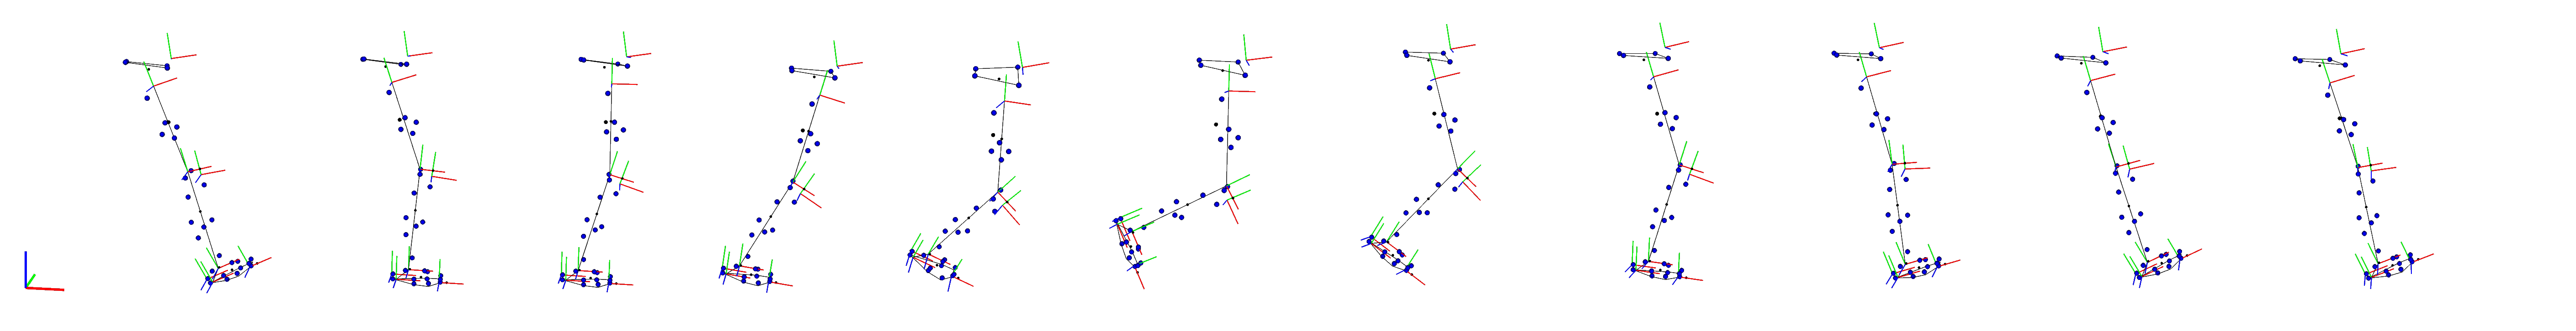
\includegraphics[width=\textwidth]{figures/multiphase_walking_cycle.png}\\
\caption{Snapshots of a walking gait cycle driven by muscles activation.}
\label{fig:snapshots_multiphase_walking_cycle}
\end{figure*}

\begin{figure*}[t!]
\centering
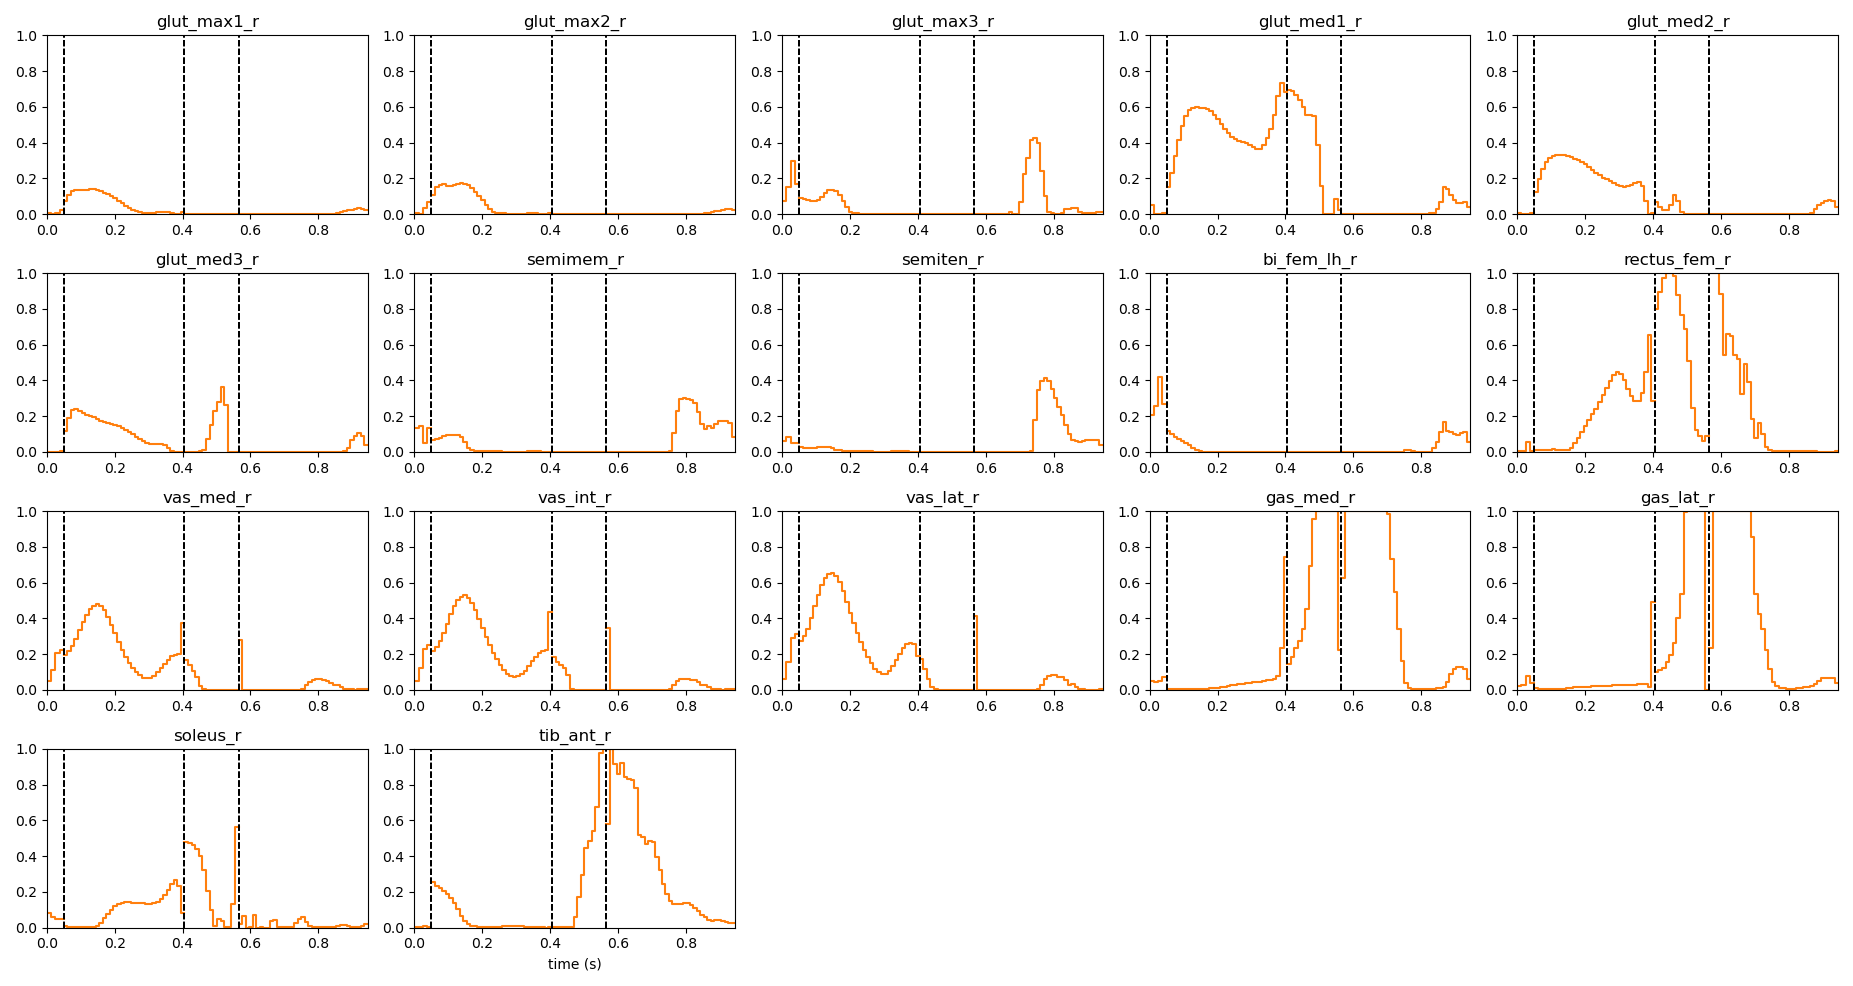
\includegraphics[width=\textwidth]{figures/muscles_control_gait_example.png}\\
\caption{Muscle activity patterns during walking cycle.}
\label{fig:muscles_activation_gait}
\end{figure*}
